
%\documentclass{article}
\documentclass[a4paper,11pt]{article}

% FILL OUT THE DETAILS BELOW:
\author{Liu Nuo Su}
\title{\textit{Thesis pre-proposal}}

\newcommand{\studentnumber}{510846}
\newcommand{\program}{Quantitative Finance}
\newcommand{\supervisor}{Dr. M. Grith}
\newcommand{\secondassesor}{TBD}

\usepackage[british]{babel} % Use British English
\usepackage[onehalfspacing]{setspace} % Increase line spacing
\usepackage[margin=2.5cm]{geometry} % Modify margins

\usepackage[hidelinks]{hyperref}
\usepackage{graphicx,booktabs,apacite} % Packages for 
\usepackage{amssymb}

%\usepackage[english]{babel}
%\usepackage[letterpaper,top=2cm,bottom=2cm,left=3cm,right=3cm,marginparwidth=1.75cm]{geometry}
\usepackage{amsmath}
\usepackage{placeins}

%\usepackage{hyperref}
%\usepackage{graphicx}
%\usepackage[colorlinks=true, allcolors=blue]{hyperref}
%\usepackage{apacite}
\usepackage{caption}
\usepackage{subcaption}
\usepackage{algpseudocode}
\usepackage{algorithm}


%\title{Thesis proposal: \textit{Extreme market volatility quantile estimation using extrapolation neural networks in a non-stationary model}}
%\author{Liu Nuo Su}

%\begin{document}
%\maketitle
\begin{document}

\begin{titlepage}
\makeatletter
\begin{center}
	\textsc{Erasmus University Rotterdam}
	\par \textsc{Erasmus School of Economics}
	\par Master Thesis \program

	\vfill \hrule height .08em \bigskip
	\par\huge\@title\bigskip
	\par\Large\@author\,(\studentnumber)\bigskip
	\hrule height .08em\normalsize
	
	\vfill
	
\includegraphics[width=\textwidth,height=0.15\textheight,keepaspectratio]{eur} % The EUR logo, but this could also be another image
	\vfill
	
	\begin{tabular}{ll}
		\toprule
		Supervisor: & \supervisor\\
		Second assessor: & \secondassesor\\
		Date final version: & \@date\\
		\bottomrule
	\end{tabular}
	
	\vfill
	The views stated in this thesis are those of the author and not necessarily those of the supervisor, second assessor, Erasmus School of Economics or Erasmus University Rotterdam.
\end{center}
\makeatother
\end{titlepage}

\tableofcontents
\pagebreak
%\begin{abstract}
%\end{abstract}
\section{Introduction} \label{introduction}
The market for ultra short tenor has grown tremendously in recent years. Since the introduction of the so-called 'weeklies', investors and traders have gained the ability to hedge against, or take advantage of short-term market trends and specific events without committing to longer-term contracts. In 2022, it is estimated that around 60\% of the daily option trading volume belonged to the ultra short term tenor options.  %[Introduction, grab attention]

Although making up the majority of the trading volume, limited research has been done on ultra short tenor options. For longer maturity derivative, researches modeling the Implied Volatility Surface (IVS) were often centered around the fundamentals of a company and the macro-economic trends at the time (e.g. \citeA{YAN2011216}, \citeA{bernales2014can}). For those derivatives, out-of-the money options are less affected by sudden market events, as volatility tends to stabilize over longer time horizons. In contrast, ultra short tenor options tend to expire within immediate market conditions, where the sudden volatility spike often ends up determining the payoff of the derivative. Therefore, ultra short tenor options are much more affected by immediate market conditions, making the predictability of the derivative much more challenging.
%such as spontaneous changes in market sentiment, earning announcements of a company, or news events. 
%In contrast, ultra short tenor options are much m
% smoothing? [IVS - and limited explain-ability in data[Describe the problem, IVS and thing]]

%[Quarterly numbers do not reflect the immediate market conditions]

In this work, we investigate the implied volatility of ultra short tenor options, and plot the options against different strike prices and times to maturity using the IVS. We employ machine learning algorithms, as they are suited for capturing complex, non-linear relations in the process of implied volatility estimation. Furthermore, as quarterly numbers do not immediately reflect the current market conditions, we incorporate news data obtained from The New York Times as explored by \cite{kim2023forecasting} as input. We make use of the FinBERT language model developed by \cite{yang2020finbert}, and is specialized to obtain the semantics of the text, use the embedding, and transform them into a format compatible for machine learning for Financial news data. 


%The price of an option is usually expressed in terms of implied volatility, as the one-to-one mapping allows for comparison of options across different strike prices and times to maturity. Plotting the volatility against the two results in the well-known IVS used by practitioners and researches alike.  %IVS here

%Furthermore, we [text data, FinBERT embedding]
%[you see them reading the news all the time]

%[machine learning]

%[Describe idea, and approach to problem - text data and Machine learning]




%[Academic and economic relevance]
From an academic standpoint, we contribute to literature investigating ultra short tenor options. We demonstrate the use of text, and we employ state of the art machine learning techniques in the context of short tenor derivatives. From an economic standpoint, the IVS is used to gauge the market sentiment at the time, and the inclusion of text data can reveal the relation between specific news events and the sentiment at the time. 

%[Research question]

In this work,  we aim to answer the following questions:
1. How useful is news data in the prediction of implied volatility surfaces of ultra short tenor options?

2. To what extend can machine learning algorithms predict the implied volatility surface of ultra short tenor derivatives?

3. What differences exist between the estimation of individual stock options and the S\&P500 index options?

[4. (Ideally) we want to make an improvement on one of the machine learning algorithms, too, and see if it is superior to the other algorithms]
[Short answer to questions]

%[Overview of the rest of the paper]
In section \ref{literature_review}, previous works on the IVS and short tenor options are investigated. Section \ref{Data} gives an overview of the data, while \ref{methods} discusses the methods used in this work.  





\section{Literature Review} \label{literature_review}

[Describe gap in literature - weekly options not researched much]

Contribution to literature:
1. Investigate the IVS on ultra short tenor options
2. Demonstrate the use of machine learning methods on the estimation of implied volatility
3. Explore the use of text data to gauge the sentiment around the stocks 

\section{Data} \label{Data}

\subsection{Ultra Short Tenor Options} \label{3_ultra_short_tenor}
[Graphs and trends in data]

\begin{figure}
    \centering
    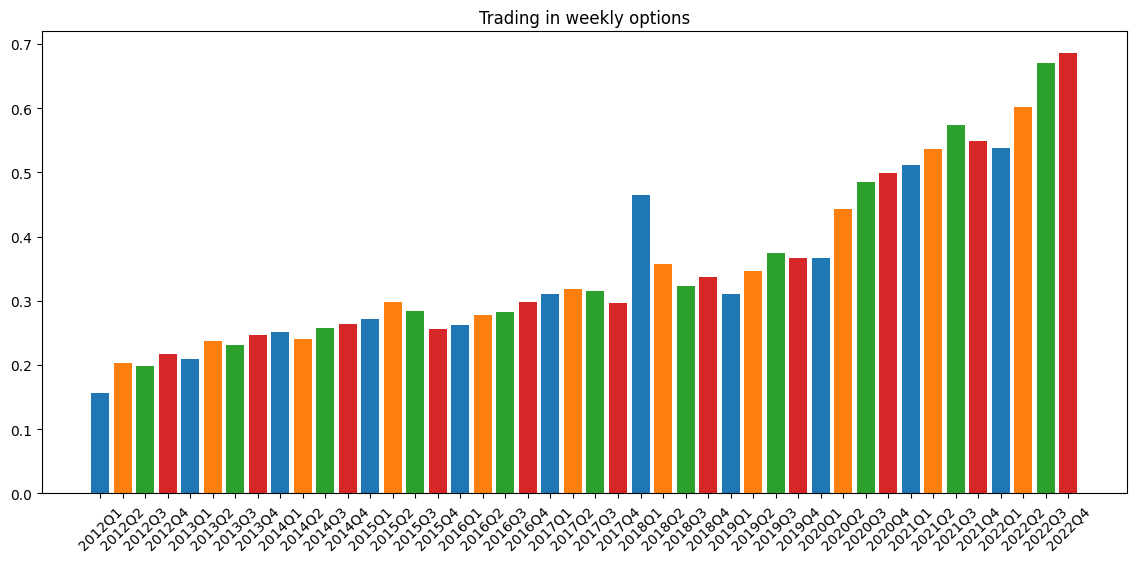
\includegraphics[width=\linewidth]{report/option_volume.png}
    \caption{Caption}
    \label{fig:enter-label}
\end{figure}
First: options data
time period, maturities, 

S\&P500 first, then individual stocks

\subsection{Macro Economic Variables and Events} \label{3_macro_data}
Second: Macro-economic variables 
Third: News and text data - FinBERT - demonstrate the embeddings

\subsection{Idiosyncratic Variables and News} \label{3_stock_data}

Then, singular stock options
- accounting variables ?

\section{Methods} \label{methods}

\subsection{Implied Volatility} \label{4_implied_vol}
[Implied volatility - how to obtain from option prices?]

\subsubsection{Black Scholes}
\subsubsection{Carr and Wu model}

\citeA{carr2016analyzing} specified a model to predict the option price, and is defined as
\begin{equation}
\begin{aligned}
    \frac{dS_{t}}{S_{t}} = \sqrt{v_{t}}dW_{t}, \\
    d\sigma_{t}(K,T) = \mu_{t}dt + \omega_{t}dZ_{t}, \\
    \text{E}[dW_{t}dZ_{t}] = \rho_{t}dt,
\end{aligned}
\end{equation}

with $[\text{log}(K/S_{t})] < \kappa$ and $0<T-t<\tau$. [work it out..]

\subsection{FinBERT}

\subsection{Machine Learning} \label{4_ML_techniques}

\subsubsection{Lasso and Ridge regression}
\subsubsection{Ensemble Methods}
\subsubsection{Support Vector Machines}
\subsubsection{Neural Network}

\subsection{Evaluation Metrics} \label{4_Evaluation_metrics}
IVRSME, R-squared, shapley values for determining feature importance


Graphs and tables obtained will depend on which evaluation metrics we want to include

\newpage
\bibliographystyle{apacite}
\bibliography{bibliography}
\appendix

\end{document}
